\chapter{ Функции теории вероятностей и математической статистики}

\section{Функции непрерывных случайных величин}
Непрерывная случайная величина задается с помощью интервала $(a,b)$ и плотности распределения вероятностей $f(x)$.
Например,  $a=0; b=2; f=1/4*x^2.$ 

Для непрерывных случайных величин  определены следующие функции:

\comm{mathExpectation}{(a, b, f(x))} вычисляет математическое ожидание непрерывной случайной величины.

\comm{dispersion}{(a, b, f(x))} вычисляет дисперсию непрерывной случайной величины. 

\comm{meanSquareDeviation}{(a, b, f(x))} вычисляет среднее квадратичное отклонение непрерывной случайной величины.

\comm{plotDistributionFunction}{(a, b, F(x))} строит функцию распределения непрерывной случайной величины, 
где  F(x) --- функция распределения на (a,b).

\underline{Примеры.}

\vspace*{-2mm}
\begin{verbatim}
SPACE=R64[x]; 
a=0;
b=4;
f=1/4;
g=\mathExpectation(a,b,f); 
g1=\dispersion(a,b,f); 
g2=\meanSquareDeviation(a,b,f);  
\print(g, g1, g2);
\end{verbatim}
%begindelete 

\ex{$SPACE=R64[x];;$\\ 
\hspace*{4mm} $a=0; b=4; f=0.25;$\\
\hspace*{4mm} $g=mathExpectation(a, b, f);$\\ 
\hspace*{4mm} $g1=dispersion(a, b, f);$\\ 
\hspace*{4mm} $g2=meanSquareDeviation(a, b, f);$\\  
\hspace*{4mm} $print(g, g1, g2);$}
{$g = 2; $\\
\hspace*{4mm} $g1 = 1.33; $\\
\hspace*{4mm} $g2 = 1.15;$} 

%enddelete
\begin{verbatim}
SPACE=R64[x];
a=0;
b=4;
F=1/16*x^2;
\plotDistributionFunction(a, b, F);
\end{verbatim}
%begindelete

\ex{$SPACE=R64[x];$\\ 
\hspace*{4mm} $a=0; b=4; F=1/16*x^2$\\
\hspace*{4mm} $plotDistributionFunction(a, b, F);$}{рис. \ref{8_2}.}
                       
\begin{figure}[!ht]
 \includegraphics[width=300.57pt, height=192.835pt]{pictures/8_2}
\caption{Функция распределения непрерывной случайной величины из примера 2}
\label{8_2}
\end{figure}
%enddelete

\section{Функции дискретных случайных величин}
Дискретная случайная величина задается как  матрица,  имеющая две строки.  В первой строке записаны значения случайной величины,  во второй~--- соответствующие им вероятности.  То есть каждый элемент второй строки является числом на отрезке [$0$,  $1$], при  этом и сумма всех элементов второй  строки должна быть равна $1$.  
Например,  $DRQ=([1, 2, 3, 4, 5], [0.4, 0.1, 0.1, 0.2, 0.2]).$ 


Для дискретных случайных величин  определены следующие функции. 

\comm{mathExpectation}{(DRQ)} вычисляет математическое ожидание дискретной случайной величины $DRQ$. 

\comm{dispersion}{(DRQ)} вычисляет дисперсию дискретной случайной величины $DRQ$. 

\comm{meanSquareDeviation}{(DRQ)} вычисляет среднее квадратичное отклонение дискретной случайной величины $DRQ$. 

\comm{addQU}{(DRQ1, DRQ2)} складывает две дискретные случайные величины $DRQ1$ и $DRQ2$. 

\comm{multiplyQU}{(DRQ1, DRQ2)} умножает две дискретные случайные величины $DRQ1$ и $DRQ2$. 

\comm{covariance}{(DRQ1, DRQ2)} вычисляет коэффициент ковариации двух дискретных случайных величин $DRQ1$ и $DRQ2$. 

\comm{correlation}{(DRQ1, DRQ2)} вычисляет коэффициент корреляции двух дискретных случайных величин $DRQ1$ и $DRQ2$. 

\comm{plotPolygonDistribution}{(DRQ)} строит многоугольник распределения дискретной случайной величины $DRQ$. 

\comm{plotDistributionFunction}{(DRQ)} строит функцию распределения дискретной случайной величины $DRQ$. 

\comm{simplifyQU}{(DRQ)} упрощает дискретную случайную величину $DRQ$. 

\underline{Примеры.}

\vspace*{-2mm}
\begin{verbatim}
SPACE=R64[x]; 
DRQ=[[1, 2], [0.2, 0.8]];
g=\mathExpectation(DRQ); 
g1=\dispersion(DRQ); 
g2=\meanSquareDeviation(DRQ);  
\print(g, g1, g2);
\end{verbatim}
%begindelete 

\ex{$SPACE=R64[x];;$\\ 
\hspace*{4mm} $DRQ=\left(\begin{array}{cc}1& 2\\ 0.2& 0.8 \end{array}\right);$\\
\hspace*{4mm} $g=mathExpectation(DRQ);$\\ 
\hspace*{4mm} $g1=dispersion(DRQ);$\\ 
\hspace*{4mm} $g2=meanSquareDeviation(DRQ);$\\  
\hspace*{4mm} $print(g, g1, g2);$}
{$g = 1. 8; $\\
\hspace*{4mm} $g1 = 0.16; $\\
\hspace*{4mm} $g2 = 0.39;$} 

%enddelete
\begin{verbatim}
SPACE=R64[x]; 
DRQ=[[7, 5, 3, 5, 1], [0.2, 0.1, 0.3, 0.1, 0.3]];
g=\simplifyQU(DRQ); 
\print(g);
\end{verbatim}
%begindelete

\ex{$SPACE=R64[x];$\\ 
\hspace*{4mm} $DRQ=\left(\begin{array}{ccccc}   7& 5& 3& 5& 1\\ 0.2& 0.1& 0.3& 0.1& 0.3 \end{array}\right);$\\
\hspace*{4mm} $g=simplifyQU(DRQ);$\\ 
\hspace*{4mm} $print(g);$
}
{$g =\left(\begin{array}{cccc}1 &3 &5 &7 \\ 0.3 &0.3 &0.2 &0.2 \end{array}\right);$}

%enddelete
\begin{verbatim}
SPACE=R64[x]; 
DRQ1=[[0, 1], [0.33333, 0.66666]]; 
DRQ2=[[1, 2], [0.25, 0.75]];
g=\addQU(DRQ1, DRQ2); 
g1= \multiplyQU(DRQ1, DRQ2);  
\print(g, g1);
\end{verbatim}
%begindelete

\ex{$SPACE=R64[x];$\\ 
\hspace*{4mm} $DRQ1=\left(\begin{array}{cc} 0& 1\\ 0.33333& 0.66666  \end{array}\right); $\\
\hspace*{4mm} $DRQ2=\left(\begin{array}{cc} 1& 2\\ 0.25& 0.75 \end{array}\right);$\\
\hspace*{4mm} $g=addQU(DRQ1, DRQ2); $\\
\hspace*{4mm} $g1= multiplyQU(DRQ1, DRQ2); $\\ 
\hspace*{4mm} $print(g, g1);$}
{$g =\left(\begin{array}{ccc}1 & 2 & 3\\ 0.08 &0.41 &0.49 \end{array}\right) ; $\\
\hspace*{4mm} $g1 =\left(\begin{array}{ccc}0 & 1 & 2\\ 0.33 &0.16 &0.49 \end{array}\right);$} 

%enddelete
\begin{verbatim}
SPACE=R64[x];
DRQ=[[-7, -2, 0, 3, 5, 7, 9], 
  [0.3, 0.05, 0.2, 0.1, 0.1, 0.2, 0.05]];
\plotPolygonDistribution(DRQ);
\end{verbatim}
%begindelete


\ex{$SPACE=R64[x];$\\ 
\hspace*{4mm} $DRQ=\left(\begin{array}{ccccccc} -7& -2& 0& 3& 5& 7& 9\\ 0.3& 0.05& 0.2& 0.1& 0.1& 0.2& 0.05 \end{array}\right);$\\
\hspace*{4mm} $plotPolygonDistribution(DRQ);$}{рис. \ref{8_1}.}
                       
\begin{figure}[!ht]
 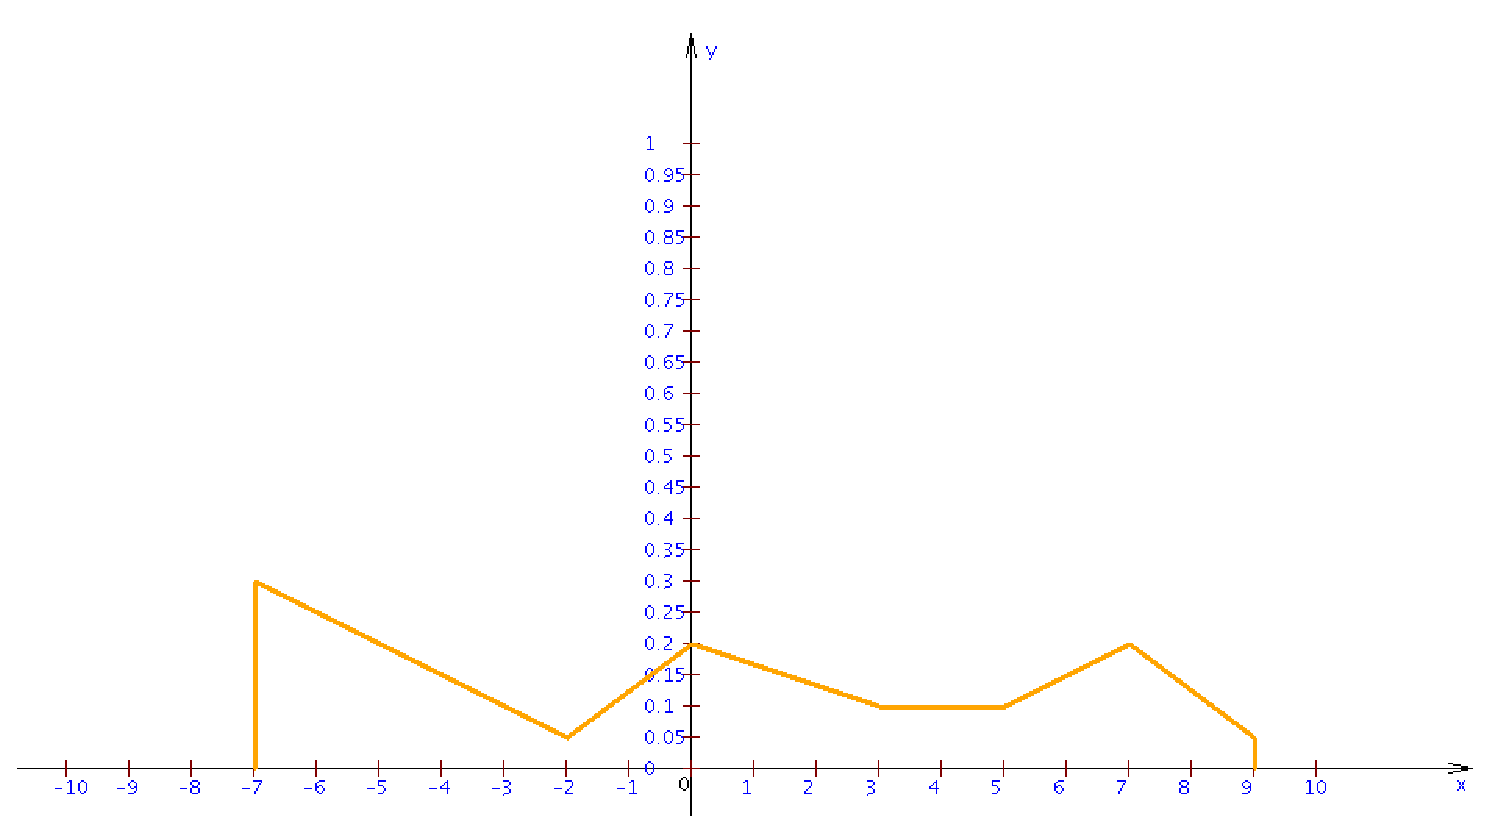
\includegraphics[width=300.57pt, height=192.835pt]{pictures/8_1}
\caption{Многоугольник распределения дискретной случайной величины из примера 4}
\label{8_1}
\end{figure}
%enddelete

\section{Функции для выборок}

Выборка задается как матрица из одной строки.  Например,  $[1, 7, 10, 15]$. 

\comm{sampleMean}{(S)} вычисляет выборочное среднее выборки $S$. 

\comm{sampleDispersion}{(S)} вычисляет выборочную дисперсию выборки $S$. 

\comm{covarianceCoefficient}{(S1, S2)} вычисляет коэффициент ковариации для 2 выборoк $S1$ и $S2$. 

\comm{correlationCoefficient}{(S1, S2)} вычисляет коэффициент корреляции для 2 выборoк $S1$ и $S2$. 

\underline{Пример. }

\vspace*{-2mm}
\begin{verbatim}
SPACE=R64[x];
S1=[0, 1]; 
S2=[1, 2];
g=\sampleMean(S1); 
g1=\sampleDispersion(S1); 
g2=\covarianceCoefficient(S1, S2); 
g3=\correlationCoefficient(S1, S2); 
\print(g, g1, g2, g3);
\end{verbatim} 
%begindelete

\ex{$SPACE=R64[x];$\\
\hspace*{4mm} $S1=[0, 1];$\\ 
\hspace*{4mm} $S2=[1, 2];$\\
\hspace*{4mm} $g=sampleMean(S1); $\\
\hspace*{4mm} $g1=sampleDispersion(S1); $\\
\hspace*{4mm} $g2=covarianceCoefficient(S1, S2); $\\
\hspace*{4mm} $g3=correlationCoefficient(S1, S2);$\\ 
\hspace*{4mm} $print(g, g1, g2, g3);$}
{$g = 0. 5; $\\
\hspace*{4mm} $g1 = 0.25; $\\
\hspace*{4mm} $g2 = 0.25; $\\
\hspace*{4mm} $g3 = 1.00$.} 
 
\section{Контрольные задания}
Заданы дискретные случайные величины $M$ и $K$\\
\begin{tabular}{c|c}
$M$&$K$\\
1 \hspace*{3mm} 1. 2 \hspace*{3mm} 1. 4 \hspace*{3mm} 1. 6 \hspace*{3mm} 1. 8\hspace*{3mm} & \hspace*{3mm} 0. 9 \hspace*{3mm} 1. 0 \hspace*{3mm} 1. 1 \hspace*{3mm} 1. 2 \hspace*{3mm} 1. 3\\
0. 1 \hspace*{1mm} 0. 1 \hspace*{3mm} 0. 3 \hspace*{3mm} 0. 4 \hspace*{3mm} 0. 1\hspace*{3mm} & \hspace*{3mm} 0. 2 \hspace*{3mm} 0. 3 \hspace*{3mm} 0. 2 \hspace*{3mm} 0. 2 \hspace*{5mm} 0. 1\\
\end{tabular}

В Mathpar найдите

\begin{itemize}
  \item математическое ожидание случайных величин $M$ и $K$, 
  \item дисперсию  случайных величин $M$ и $K$, 
  \item среднее квадратичное отклонение  случайных величин $M$ и $K$, 
  \item сумму,  произведение  случайных величин $M$ и $K$, 
  \item коэффициент ковариации  случайных величин $M$ и $K$, 
  \item коэффициент корреляции  случайных величин $M$ и $K$. 
  \item Постройте многоугольник распределения дискретной случайной величины $M$ и ее функции распределения. 
\end{itemize}
%enddelete
